\begin{figure}[!htbp]
  \centering
  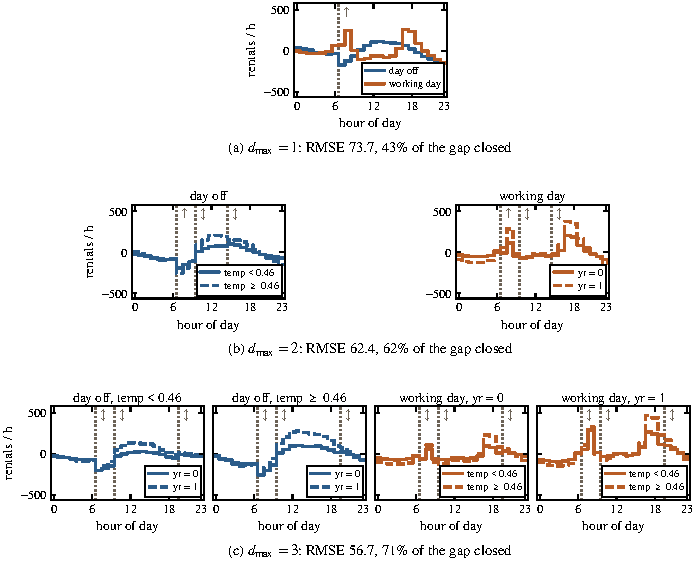
\includegraphics[width=\linewidth]{images/ladder}
  \caption{What depth buys: the hour of the Bike Sharing data under \method{} at $d_{\max} = 1$, $2$ and $3$ (fits on all rows; depth 1 is the model of Figure~\ref{fig:hero}, depth 2 the default of Table~\ref{tab:regr-rmse}).
    Each level splits every region once more, giving $2$, $4$ and $8$ curves: (a) shows both, (b) one panel per day type and (c) one panel per region of the first two splits, each panel above the two it splits into; the hue is the day type, the line style the last split; dotted lines mark where another feature's region switches on the hour, each with the sign of its hidden jump (\S\ref{subsec:interpretability-properties}): $\uparrow$~$[36, 334]$ at depth 1; $\uparrow$~$[8, 267]$, $\updownarrow$~$[-159, 63]$ and $\updownarrow$~$[-48, 70]$ at depth 2; all three $\updownarrow$ at depth 3.
    Under each depth, the held-out RMSE of that depth and the share of the GAM\,$\to$\,XGBoost gap it closes, over 5 folds (GAM 100.2, XGBoost 39.4): 43\,\%, 62\,\% and 71\,\%.}
  \label{fig:ladder}
\end{figure}
